
\chapter{Data Processing and Visualization}
\label{chap:tabgenie}
% \section{Motivation}
% \label{sec:data-mot}
\section{TabGenie Toolkit}
\label{sec:tabgenie}

\begin{refbox}
    This section is based on the paper \emph{\textsc{TabGenie}: A Toolkit for Table-to-Text Generation} \cite{kasnerTabGenieToolkitTabletoText2023}, joint work with Ekaterina Garanina, Ondřej Plátek, and Ondřej Dušek. The work was published as a system demonstration in the Proceedings of the 61st Annual Meeting of the Association for Computational Linguistics (ACL 2023). The project was led by the author of the thesis, the remaining authors helped with implementing the framework and paper writing.
\end{refbox}

Heterogenity of data-to-text generation datasets limits the research on data-to-text generation systems. We present \textsc{TabGenie} -- a toolkit which enables researchers to explore, preprocess, and analyze a variety of data-to-text generation datasets through the unified framework of \textit{table-to-text generation}. In \textsc{TabGenie}, all inputs are represented as tables with associated metadata. The tables can be explored through a web interface, which also provides an interactive mode for debugging table-to-text generation, facilitates side-by-side comparison of generated system outputs, and allows easy exports for manual analysis. Furthermore, \textsc{TabGenie} is equipped with command line processing tools and Python bindings for unified dataset loading and processing. We release \textsc{TabGenie} as a PyPI package\footnote{\url{https://pypi.org/project/tabgenie/}} and provide its open-source code and a live demo at \url{https://github.com/kasnerz/tabgenie}.

Building and evaluating data-to-text (D2T) generation systems \cite{gatt2018survey,sharma2022innovations} requires understanding the data and observing system behavior. It is, however, not trivial to interact with the large volume of D2T generation datasets that have emerged in the last years (see Table~\ref{tab:datasets}).
Although research on D2T generation benefits from platforms providing unified interfaces, such as HuggingFace Datasets \cite{lhoest2021datasets} or the GEM benchmark \cite{gehrmann2021gem}, these platforms still leave the majority of the data processing load on the user.

A key component missing from current D2T tools is the possibility to visualize the input data and generated outputs. Visualization plays an important role in examining and evaluating scientific data \cite{Kehrer2013VisualizationAV} and can help D2T generation researchers to make more informed design choices. A suitable interface can also encourage researchers to step away from unreliable automatic metrics \cite{gehrmann2022repairing} and focus on manual error analysis \cite{van_miltenburg_underreporting_2021,van_miltenburg_barriers_2023}.

Along with that, demands for a \textit{unified input data format} have recently been raised with multi-task training for large language models (LLMs) \citep[\textit{inter alia}]{Sanh2021MultitaskPT,scao2022bloom,Ouyang2022TrainingLM}. Some works have used simple data linearization techniques for converting structured data to a textual format, in order to align it with the format used for other tasks \cite{UnifiedSKG,tang2022mvp}. However,  linearizations are using custom preprocessing code, leading to discrepancies between individual works.


In this paper, we present \textsc{TabGenie} -- a multi-purpose toolkit for interacting with D2T generation datasets and systems designed to fill these gaps. On a high level, the toolkit consists of (a) an interactive web interface, (b) a set of command-line processing tools, and (c) a set of Python bindings (see Figure~\ref{fig:teaser}).


The cornerstone of \textsc{TabGenie} is a \textbf{unified data representation}. Each input represented is as a matrix of $m$ columns and $n$ rows consisting of individual cells accompanied with metadata (see §\ref{sec:data}). Building upon this representation, \textsc{TabGenie} then provides multiple features for unified workflows with table-to-text datasets, including:
\begin{enumerate}
    \item visualizing individual dataset examples in the tabular format (§\ref{sec:exploration}),
    \item interacting with table-to-text generation systems in real-time (§\ref{sec:interactive}),
    \item comparing generated system outputs (§\ref{sec:interactive}),
    \item loading and preprocessing data for downstream tasks (§\ref{sec:python}),
    \item exporting examples and generating spreadsheets for manual error analysis (§\ref{sec:cli}).
\end{enumerate}

In §\ref{sec:casestudies}, we present examples of practical use-cases of \textsc{TabGenie} in D2T generation research.

\subsection{Data}
\label{sec:tabgenie:data}
We currently include 16 datasets listed in Table~\ref{tab:datasets} in \textsc{TabGenie}, covering many subtasks of D2T generation. All the datasets are available under a permissive open-source license.

\begin{figure*}[t]
    \centering
    \setlength{\fboxsep}{0pt}\fcolorbox{gray!20}{white}{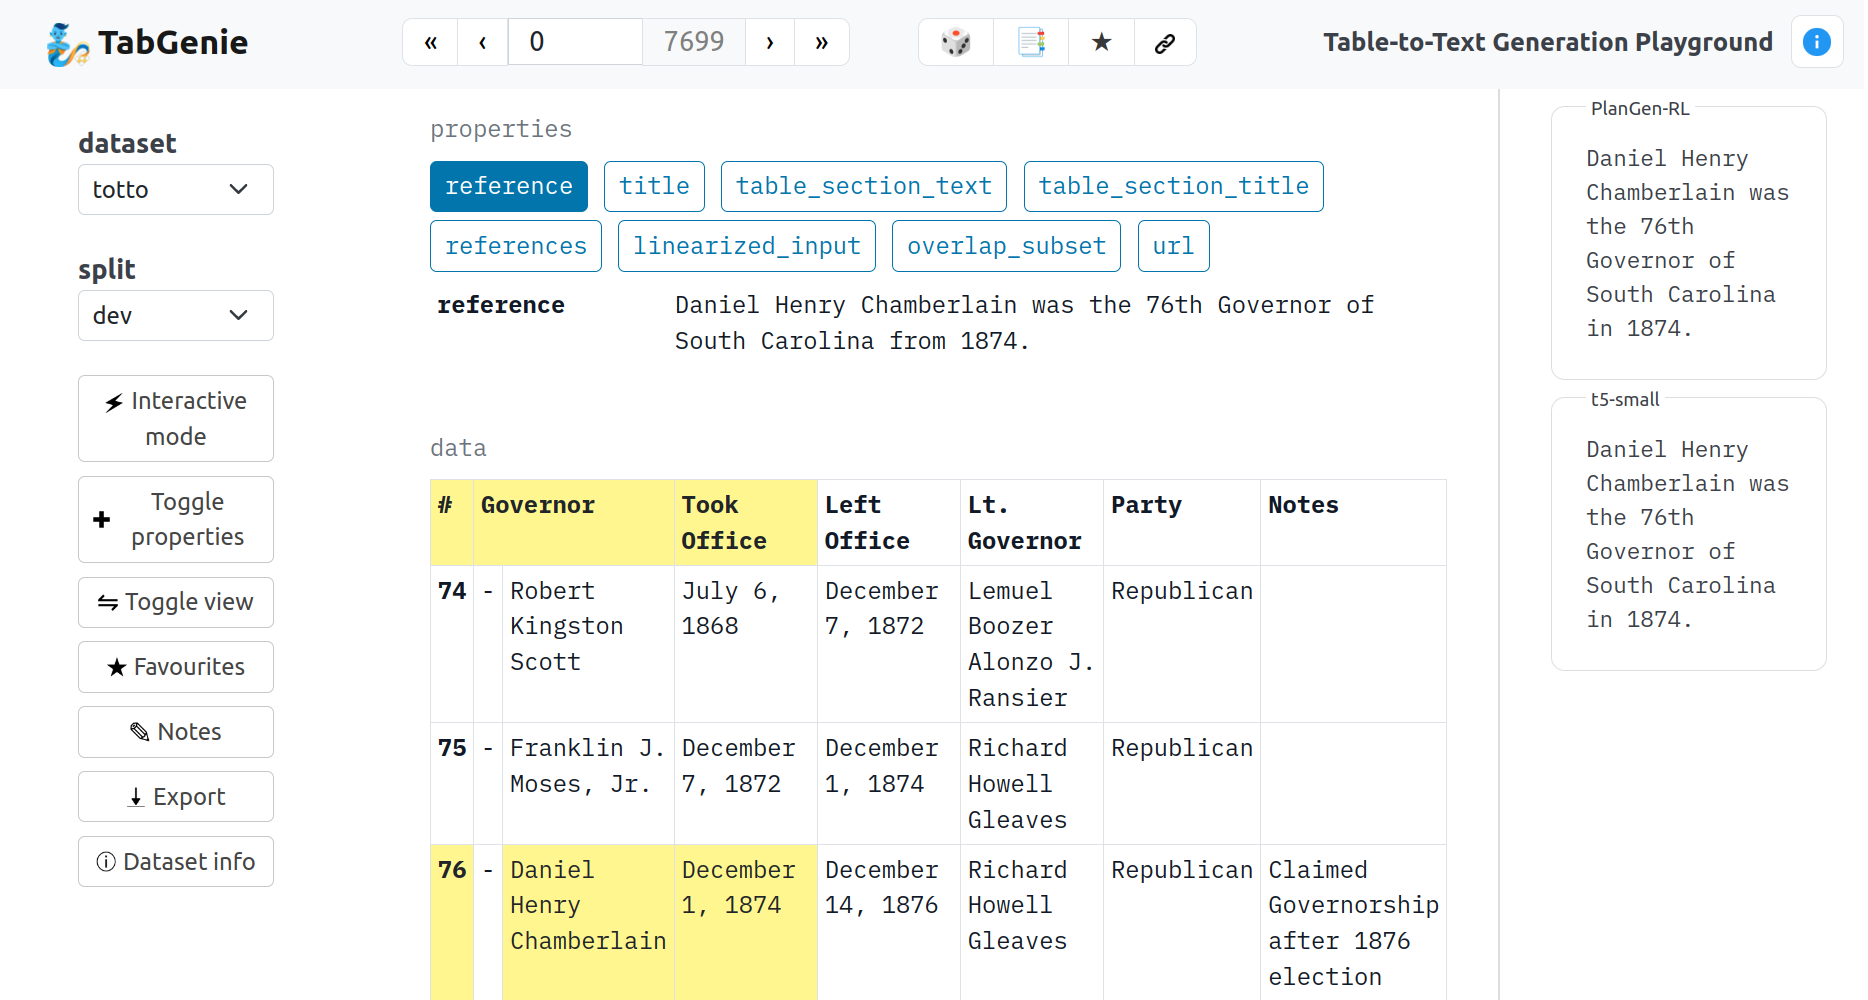
\includegraphics[width=1.0\textwidth]{img/tabgenie_web.png}}
    \caption{The web interface of \textsc{TabGenie}. The \textbf{left panel} and the \textbf{navigation bar} contains user controls; the \textbf{center panel} shows table properties and table content; the \textbf{right panel} contains system outputs.}
    \label{fig:web}
\end{figure*}


\subsection{Data Format}
The inputs in D2T generation datasets may not consist only of tables, but also of e.g.\ graphs or key-value pairs. However, we noticed that in many cases, converting these formats to tables requires only minimal changes to the data structure while allowing a unified data representation and visualization. This conversion narrows down the task of D2T generation as the task of generating description for a tabular data, i.e. table-to-text generation \cite{parikh2020totto, liu2022plog, gong2020tablegpt}.


In our definition, a \textit{table} is a two-dimensional matrix with $m$ columns and $n$ rows, which together define a grid of $m \times n$ cells. Each cell contains a (possibly empty) text string. A continuous sequence of cells $\{c_{i}, \ldots, c_{i+k}\}$ from the same row or column may be merged, in which case the values of $\{c_{i+1},\ldots,c_{i+k}\}$ are linked to the value of $c_{i}$.  A cell may be optionally marked as a \textit{heading}, which is represented as an additional property of the cell.\footnote{The headings are typically located in the first row or column, but may also span multiple rows or columns and may not be adjacent.} To better accommodate the format of datasets such as ToTTo \cite{parikh2020totto} or HiTab \cite{cheng2021hitab}, we also allow individual cells to be \textit{highlighted}. Highlighted cells are assumed to be preselected for generating the output description.


The tables may be accompanied with an additional set of properties (see Figure~\ref{fig:web}) -- an example of such a property is a \textit{``title''} of the table in WikiBio \cite{lebret2016neural} or a \textit{``category''} in WebNLG \cite{gardent2017webnlg}. We represent properties as key-value pairs alongside the table. The properties may be used for generating the table description.

\paragraph{Data Transformation}
We aim to present the data as true to the original format as possible and only make some minor changes for datasets which do not immediately adhere to the tabular format:

\begin{itemize}
    \item For graph-to-text datasets, we format each triple as a row, using three columns labeled \textit{subject}, \textit{predicate}, and \textit{object}.
    \item For key-value datasets, we use two columns with keys in the first column as row headings.
    \item For SportSett:Basketball \cite{thomson-etal-2020-sportsett}, we merge the \textit{box score} and \textit{line score} tables and add appropriate headings where necessary.
\end{itemize}

Moreover, for ToTTo \citep{parikh2020totto}, we also provide our custom, improved header cells highlighting (details are given in Appendix \ref{appendix:totto_highlights}).


\paragraph{Data Loading}
To ease the data distribution, we load all the datasets using the Huggingface \texttt{datasets} package \cite{lhoest2021datasets}, which comes equipped with a data downloader. Out of 16 datasets we are using, 7 were already available in Huggingface datasets, either through the GEM benchmark \cite{gehrmann2021gem} or other sources. We publicly added the 9 remaining datasets (see Table~\ref{tab:datasets}).


\textsc{TabGenie} also supports adding custom data loaders. Creating a data loader consists of simple sub-classing the data loader class and overriding a single method for processing individual entries, allowing anyone to add their custom dataset.

\subsection{Web Interface}
\label{sec:tabgenie:web}

\textsc{TabGenie} offers a user-friendly way to interact with table-to-text generation datasets through the \textit{web interface}. The interface can be rendered using a local server (cf. §\ref{sec:cli}) and can be viewed in any modern web browser. The interface features a simple, single-page layout, which contains a navigation bar and three panels containing user controls, input data, and system outputs (see Figure \ref{fig:web}). Although the interface primarily aims at researchers, it can be also used by non-expert users.



\paragraph{Content Exploration}
\textsc{TabGenie} renders input data as HTML tables. This approach provides superior visualizations to existing data viewers, especially in the case of large and hierarchical tables.\footnote{Compare, e.g., with the ToTTo dataset in Huggingface Datasets for which the table is provided in a single field called \textit{``table''}: \url{https://huggingface.co/datasets/totto}}

In the web interface, users can navigate through individual examples in the dataset sequentially, access an example using its index, or go to a random example. The users can add notes to examples and mark examples as favorites for accessing them later. The interface also shows the information about the dataset (such as its description, version, homepage, and license) and provides an option to export the individual examples (see §\ref{sec:cli}).



\paragraph{Interactive Mode}
\textsc{TabGenie} offers an \textit{interactive mode} for generating an output for a particular example on-the-fly. The user can highlight different cells, edit cell contents, and edit parameters of the downstream processor. For example, the user can prompt a LLM for table-to-text generation and observe how it behaves while changing the prompt.

The contents of a table are processed by a processing \textit{pipeline}. This pipeline takes table contents and properties as input, processes them with a sequence of modules, and outputs HTML code. The modules are custom Python programs which may be re-used across the pipelines.

\textsc{TabGenie} currently provides two basic pipelines: (1) calling a generative language model through an API with a custom prompt, and (2) generating graph visualizations of RDF triples. We describe a case-study for the model API pipeline in §\ref{sec:cs:prompting}. Users can easily add custom pipelines by following the instructions in the project repository.

\paragraph{Pre-generated Outputs}
In addition to interactive generation, \textsc{TabGenie} allows users to visualize static pre-generated outputs. These are loaded in the JSONL\footnote{\url{https://jsonlines.org}} format from a specified directory and displayed similarly to model-generated outputs from the interactive mode. Multiple outputs can be displayed alongside a specific example, allowing to compare outputs from multiple systems.


\subsection{Developer Tools}
\label{sec:tabgenie:developer}

\textsc{TabGenie} also provides a developer-friendly interface: Python bindings (§\ref{sec:python}) and a command-line interface (§\ref{sec:cli}). Both of these interfaces aim to simplify dataset preprocessing in downstream tasks. The key benefit of using \textsc{TabGenie} is that it provides streamlined access to data in a consistent format, removing the need for dataset-specific code for extracting information such as table properties, references, or individual cell values.



\paragraph{Python Bindings}
\textsc{TabGenie} can be integrated in other Python codebases to replace custom preprocessing code. With a \textit{single unified interface} for all the datasets, the \textsc{TabGenie} wrapper class allows to:
\begin{itemize}
    \item load a dataset from the Huggingface Datasets or from a local folder,
    \item access individual table cells and their properties,
    \item linearize tables using pre-defined or custom functions,
    \item prepare the Huggingface \texttt{Dataset} objects for downstream processing.
\end{itemize}
\textsc{TabGenie} can be installed as a Python package, making the integration simple and intuitive.
See §\ref{sec:cs:generation} for an example usage of the \textsc{TabGenie} Python interface.


\paragraph{Command-line Tools}
\textsc{TabGenie} supports several basic commands via command line.

\paragraph{Run} The \texttt{tabgenie run} command launches the local web server, mimicking the behavior of \texttt{flask run}. Example usage:

\begin{python}
    tabgenie run --port=8890 --host="0.0.0.0"
\end{python}

\paragraph{Export} The \texttt{tabgenie export} command enables batch exporting of the dataset. The supported formats are \texttt{xlsx}, \texttt{html}, \texttt{json}, \texttt{txt}, and \texttt{csv}. Except for \texttt{csv}, table properties can be exported along with the table content. Example usage:

\begin{python}
    tabgenie export --dataset "webnlg" \
    --split "dev" \
    --out_dir "export/datasets/webnlg" \
    --export_format "xlsx"
\end{python}
\noindent Export can also be done in the web interface.

\paragraph{Spreadsheet} For error analysis, it is common to select $N$ random examples from the dataset along with the system outputs and manually annotate them with error categories (see~§\ref{sec:cs:analysis}). The \texttt{tabgenie sheet} command generates a suitable spreadsheet for this procedure. Example usage:

\begin{python}
    tabgenie sheet --dataset "webnlg" \
    --split "dev" \
    --in_file "out-t5-base.jsonl" \
    --out_file "analysis_webnlg.xlsx" \
    --count 50
\end{python}

